\documentclass{beamer}
\usepackage{lsfolien,enumitem}
\usepackage[english]{babel}

\myfootline{System Modelling and Semantic Web -- Spring 2021}{Hans-Gert Gräbe}

\newcommand{\ueberschrift}[1]{\begin{center}\bf #1\end{center}}

\title{Modelling Sustainable Systems\\ and Semantic Web\\[6pt] Technology
  \vskip1em}

\subtitle{Lecture in the Module 10-202-2309\\ for Master Computer Science}

\author{Prof. Dr. Hans-Gert Gräbe\\
\url{http://www.informatik.uni-leipzig.de/~graebe}}

\date{April 2021}
\begin{document}

{\setbeamertemplate{footline}{}
\begin{frame}
  \titlepage
\end{frame}}

\section{Background}
\begin{frame}{What is Technology?}

Technology in the sense of the \textbf{VDI Guideline 3780} comprises:
\begin{itemize}
\item[-] the set of use-oriented, artificial, representational structures
  (artefacts or material systems),
\item[-] the set of human actions and facilities in which material systems
  (Sachsysteme) are created and
\item[-] the set of human actions in which material systems are used.
\end{itemize}

  \textbf{Technology assessment} thus refers not only to material real-world
  systems, but also to the conditions and consequences of their creation and
  use.
\end{frame}

\begin{frame}{Definition of Technology -- Purpose and Objective}

The \textbf{target group} of the VDI Guideline 3780 is all those responsible
and affected in science, society and politics, who are involved in decisions
about technical developments and in shaping the corresponding socio-cultural
framework conditions, in particular engineers, scientists, planners and
managers who design and evaluate new technical developments.

The \textbf{purpose} of the guideline is to provide all those involved with a
common understanding of terms, methods and value ranges. The guideline is
intended to systematically analyse objectives, values and alternatives to make
well-founded decisions. ...

\end{frame}

\begin{frame}{Technology excites}

  \begin{minipage}{.45\textwidth}\centering   
      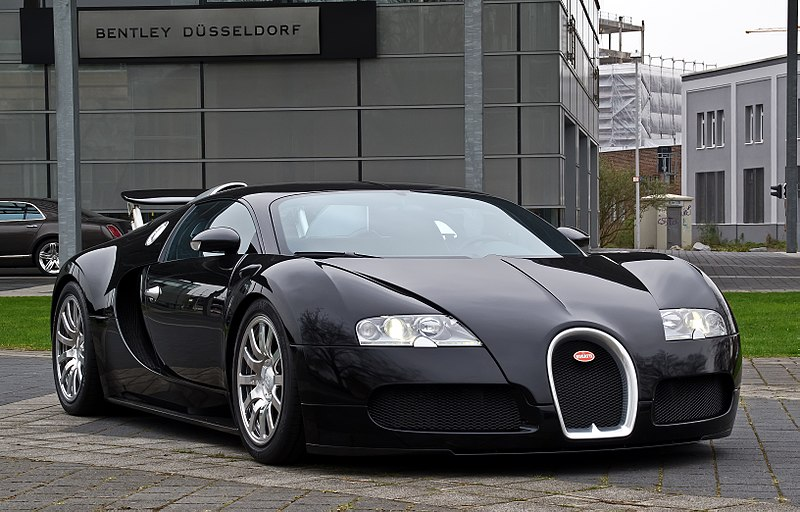
\includegraphics[width=.9\textwidth]{Bugatti.jpg} 
  \end{minipage}\hfill
  \begin{minipage}{.5\textwidth}\raggedright
    Technology as a status symbol\vskip1em

    But: You find there also detailed description of the technical parameters
    and the history.
  \end{minipage}
  
\vskip1em\small  
Source: \url{http://de.wikipedia.org/wiki/Bugatti_Veyron_16.4}


\end{frame}

\begin{frame}{Technology excites?}


  \begin{minipage}{.45\textwidth}\centering   
  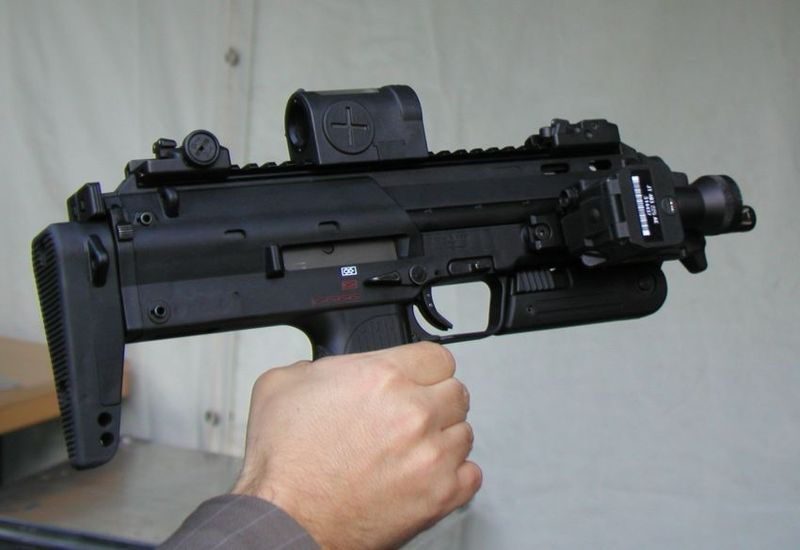
\includegraphics[width=.9\textwidth]{Maschinenpistole.jpg} 
  \end{minipage}\hfill
  \begin{minipage}{.5\textwidth}\centering   \small
    "Weapons from the 3D printer"\\ Source: Netzpolitik.org, 29.3.2013
  \end{minipage}\vskip1em\small
  
\begin{quote}
  ... In the meantime, statistics show that most of military combats take place
  at distances of less than 400 m, even less than 200 m in urban areas. In the
  case of police operations, the distances are usually even shorter.  At the
  same time, the shooter is no longer in the open field, but often fights from
  vehicles or inside buildings, where only compact weapons offer sufficient room
  for movement. ...
\end{quote}
Source: \url{http://de.wikipedia.org/wiki/Maschinenpistole}

\end{frame}

\begin{frame}{What else is Technology?}

  Technology is about techniques (in German oft the same word „Technik“ is
  used for both notions)
  
  \begin{itemize}
  \item[-] Painting techniques, writing techniques
  \item[-] Flower arranging techniques
  \item[-] Political techniques, power techniques
  \end{itemize}

  \begin{center}\Large
    $\Rightarrow$ It is about Practice, Experience, Skill
  \end{center}
Different variants of a machine-centered and an action-centered understanding
of technology compete with each other.

\end{frame}

\begin{frame}{More on the Concept of Technology}

1) The concept of technology for products of technically supported action,
i.e. for individual machines or, more comprehensively, for the entire existing
system of material means to transform nature for human purposes.

2) An action-oriented concept of technology ... ties in with the Greek concept
of \emph{techné} as procedural knowledge that guides people in the production
of things ... and thus enables a technical knowledge that controls nature in
both a reproductive and a manipulative sense. (Source: H. Petzold, Dictionary
of Philosophy)

\end{frame}

\begin{frame}{Technology and Language}

Technique is something that obeys to the word.

Example: Sven-Åke Johansson - Concerto for 12 Tractors

Picture source: Höfgen 1996, Photo: Bahr,
\url{http://www.sven-akejohansson.com}

\begin{center}
  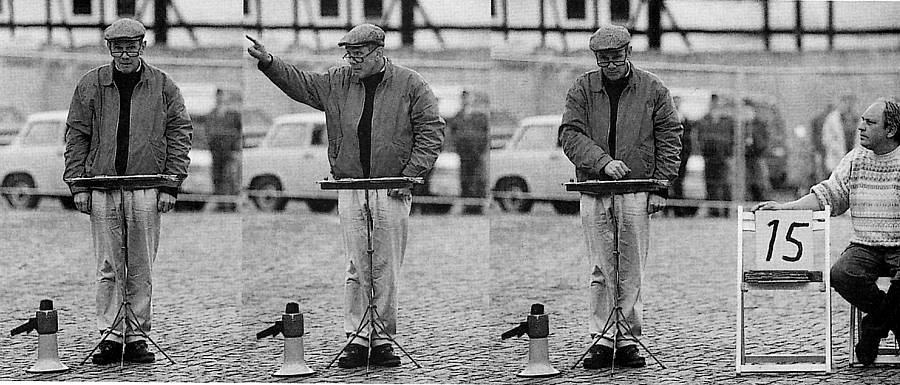
\includegraphics[width=.74\textwidth]{6lxSq6.jpg}\hfill
  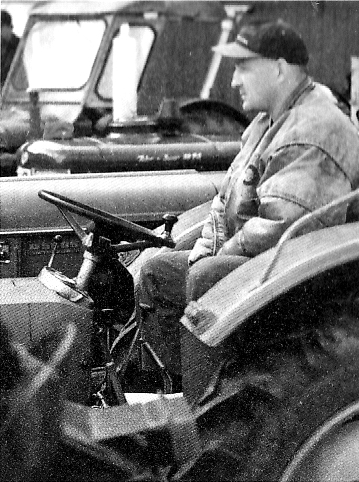
\includegraphics[width=.24\textwidth]{6barSY.jpg}
\end{center}

\end{frame}

\begin{frame}{Technology and Forms of Description}
  \begin{itemize}
  \item[-] Technology as "condensed“ description
  \item[-] Essential form in which human agreements manifest theirself
  \item[-] Technology as a social phenomenon of humanity
  \item[-] Technology as an intersubjective phenomenon
  \item[-] Essential intersubjective dimensions: Descriptions and execution of
    action
  \end{itemize}
  \begin{block}{What is Technology?} 
    Technology is an interrelation of
    \begin{itemize}
    \item[$\bullet$] Socially available \emph{procedural knowledge}
      ("Verfahrenswissen"), 
    \item[$\bullet$] \emph{Institutionalised
      procedures}\\ ("Verfahrensweisen", "state of the art") and
    \item[$\bullet$] Private \emph{procedural skills} ("Verfahrenskönnen").
    \end{itemize}
  \end{block}
\end{frame}

\end{document}
